% Source: ../../Reading/ch02/scan.pdf page 4 (bottom, from "9/23 Class"), then
% scan.pdf pages 1-4.
\documentclass[11pt]{article}
\usepackage[margin=1in]{geometry}
\usepackage{parskip}
\usepackage{amsmath,amssymb}
\usepackage{booktabs}
\usepackage{graphicx}
\usepackage{xcolor}
\usepackage{tikz}
\usepackage{pgfplots}
\pgfplotsset{compat=1.18}
\usepackage[hidelinks]{hyperref}

% Uncertain reading from the scan. Prints red until you fix it against the paper.
\newcommand{\unclear}[1]{\textcolor{red}{[#1?]}}

% Explanation added during processing, not written on the page.
\newenvironment{aside}{\begin{quote}\small\color{black!65}\textbf{Note.}\ }{\end{quote}}

\title{ISE 555 Lecture Notes\\\large Feasibility, Active Constraints, and Feasible Directions}
\author{Luke Pepin}
\date{September 23, 2026}

\begin{document}
\maketitle

\section{Feasibility and Constraints}

\begin{itemize}
    \item At a specific feasible point $\bar{x}$, an inequality constraint
          $g_i(x) \ge 0$ is called \textbf{active} (or \textbf{binding}) if
          $g_i(\bar{x}) = 0$, and \textbf{inactive} (or \textbf{nonbinding}) if
          $g_i(\bar{x}) > 0$.
    \item The \textbf{active set} at a feasible point is the set of all constraints
          that are active at that point.
    \item \textbf{Boundary:} the set of all feasible points \unclear{definition left unfinished}
    \item \textbf{Interior points:} \unclear{definition left unfinished}
\end{itemize}

\subsection*{Example: feasible, active, boundary}

\begin{itemize}
    \item What constitutes a point $x$?
    \item What are the constraint functions $g_i(x)$ under ``subject to''?
    % CHANGED: page says "iota is the inequality set"; the table heading on the same
    % page and Juan's notes both use J.
    \item $\mathcal{E}$ is the equality set and $\mathcal{J}$ is the inequality set.
    \item Is $(0, 125, 50, 50)$ feasible or infeasible? Plug the point into each
          constraint to see whether it is possible.
    \item Active or inactive: a constraint is inactive if it does not hold with
          equality, but the point can still be on a boundary as defined by the
          solution space.
\end{itemize}

Take the equality constraint
\[
    g_1(x) = x_1 + 2x_2 + 3x_3 - 6 = 0.
\]
What are $\mathcal{E}$ and the set $\mathcal{J}$?

\begin{center}
\begin{tabular}{llcccc}
    \toprule
     & Point & Feasible? & Active? & Boundary? & $g_1(x)$ \\
    \midrule
    (i)   & $(0, 0, 2)^T$ & $\checkmark$ & $\checkmark$ & $\checkmark$ & 0 \\
    (ii)  & $(3, 0, 1)^T$ & $\checkmark$ & $\checkmark$ & $\checkmark$ & 0 \\
    (iii) & $(0, 2, 1)^T$ & $\times$     & $\times$     & $\times$     & 1 \\
    (iv)  & $(1, 1, 1)^T$ & $\checkmark$ & $\checkmark$ & \unclear{$\checkmark$} & 0 \\
    \bottomrule
\end{tabular}
\end{center}

Point (iii) is infeasible because $g_1(0, 2, 1) = 0 + 4 + 3 - 6 = 1 \ne 0$.

\begin{itemize}
    \item \textbf{Set $S$, feasible points:} \unclear{left blank}
    \item \textbf{Boundary:} $(0, 0, 2)$, $(3, 0, 1)$, $(4, 1, 0)$
\end{itemize}

\begin{center}
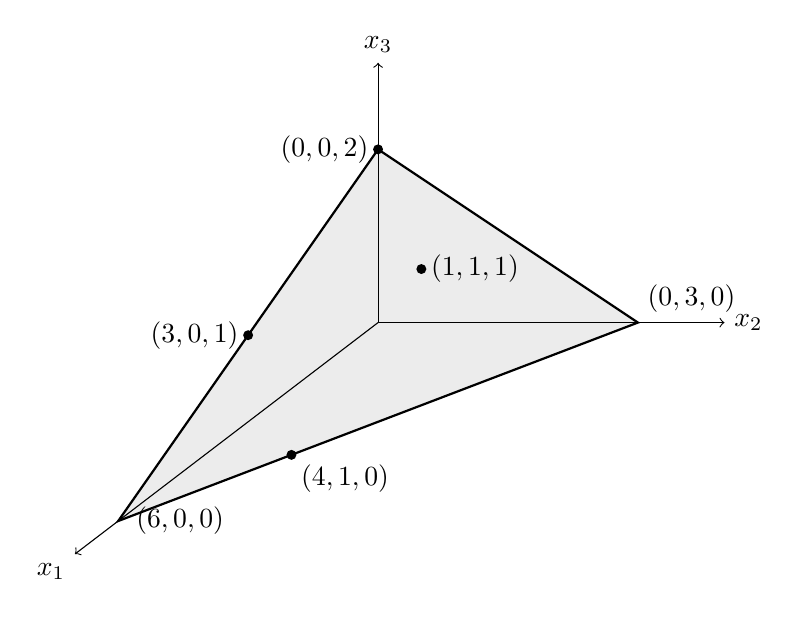
\begin{tikzpicture}[x={(-0.55cm,-0.42cm)}, y={(1.1cm,0cm)}, z={(0cm,1.1cm)}]
    \filldraw[fill=gray!15, draw=black, thick] (6,0,0) -- (0,3,0) -- (0,0,2) -- cycle;
    \draw[->] (0,0,0) -- (7,0,0) node[anchor=north east] {$x_1$};
    \draw[->] (0,0,0) -- (0,4,0) node[anchor=west] {$x_2$};
    \draw[->] (0,0,0) -- (0,0,3) node[anchor=south] {$x_3$};
    \fill (0,0,2) circle (1.8pt) node[left]  {$(0,0,2)$};
    \fill (3,0,1) circle (1.8pt) node[left]  {$(3,0,1)$};
    \fill (4,1,0) circle (1.8pt) node[below right] {$(4,1,0)$};
    \fill (1,1,1) circle (1.8pt) node[right] {$(1,1,1)$};
    \node[right=3pt] at (6,0,0) {$(6,0,0)$};
    \node[above right] at (0,3,0) {$(0,3,0)$};
\end{tikzpicture}
\end{center}

\begin{aside}
The sketch assumes the inequality constraints are $x_1, x_2, x_3 \ge 0$, which the
boundary points suggest; the page doesn't list them. The feasible set $S$ is then
the shaded triangle where the plane $g_1(x) = 0$ meets the non-negative orthant.
\end{aside}

Definitions to declare: \textbf{feasible}, \textbf{active}, \textbf{boundary}.

\emph{What is the difference between active and boundary?}

\begin{aside}
\emph{Active} describes a constraint at a point: $g_i(\bar{x}) = 0$. An equality
constraint is active at every feasible point. \emph{Boundary} describes a point: in
the usual definition, a feasible point is on the boundary if at least one
inequality constraint is active there, and it is an interior point if none are.
With $x \ge 0$ as the inequalities, $(0,0,2)$, $(3,0,1)$ and $(4,1,0)$ each have a
zero coordinate, so they are boundary points. $(1,1,1)$ has none, so under this
definition it would be interior. That is why the boundary check for (iv) is
flagged in the table above. Check it against the lecture PDF.
\end{aside}

\section{Optimization by Moving in Feasible Directions}

\begin{minipage}[t]{0.47\linewidth}
\textbf{General Algorithm I}
\begin{enumerate}
    \item Initial guess $x_0$.
    \item For $k = 0, 1, \ldots$
    \begin{itemize}
        \item If $x_k$ is optimal, stop.
        \item If not, move to $x_{k+1}$.
    \end{itemize}
\end{enumerate}
\end{minipage}\hfill
\begin{minipage}[t]{0.47\linewidth}
\textbf{General Algorithm II}
\begin{enumerate}
    \item Initial guess $x_0$.
    \item For $k = 0, 1, \ldots$
    \begin{itemize}
        \item If $x_k$ is optimal, stop.
        \item Determine a search direction $p_k$.
        \item Determine a step length $\alpha_k$.
        \item $x_{k+1} = x_k + \alpha_k p_k$.
    \end{itemize}
\end{enumerate}
\end{minipage}

\subsection{Determining the direction \texorpdfstring{$p_k$}{p\_k}}

% CHANGED: page says "descent location"; the heading and context mean direction.
For minimization, $p_k$ is called a \textbf{descent direction} if
\[
    f(x_k + \alpha p_k) < f(x_k) \qquad \text{for } 0 < \alpha \le \varepsilon,
\]
where $k$ is the step index, $\alpha p_k$ is the step (a small amount times the
direction), and $\varepsilon$ is some arbitrarily small number. In words:
``whenever we make a small step, the value is less than where we started.''

\begin{itemize}
    \item \textbf{Nonlinear} optimization is all about making constant improvement steps.
    \item \textbf{Linear} objective $f(x) = c^T x$ (plug and chug), for minimization:
    \[
        c^T x_k + \alpha c^T p_k < c^T x_k \quad\Longrightarrow\quad c^T p_k < 0.
    \]
    \item Feasible set $S$: only move in that direction if the step stays feasible.
\end{itemize}

\subsection{Feasible-point method}

% CHANGED: page labels the constraint f(x); f is the objective elsewhere in these notes.
Take the equality constraint $x_1 + x_2 = 1$, written as
\[
    c_i^T x = b_i \qquad \text{with } c_i = (1, 1)^T \text{ and } b_i = 1.
\]
If we move in direction $p$, then $c_i^T(x + \alpha p) = b_i$ only if
\[
    c_i^T p = 0, \quad\text{i.e.}\quad p_1 + p_2 = 0.
\]
% CHANGED: page says "p is the null space of c_i".
So $p$ must lie in the \textbf{null space} of $c_i^T$.

If we switch to the inequality $x_1 + x_2 \ge 1$, then we need $c_i^T p \ge 0$ to
stay feasible.

\begin{aside}
This condition matters when the inequality is active at $x$ (that is,
$x_1 + x_2 = 1$). If it is inactive, a small enough step in any direction keeps it
satisfied.
\end{aside}

The null space is important for finding feasible points around the boundary.

\subsection*{Example 1: feasible-point method}

Minimize: $2x_1 - x_2$

Subject to:
\begin{itemize}
    \item $x_1 + x_2 \le 2$
    \item $x_1, x_2 \ge 0$
\end{itemize}

Note that $f(x) = c^T x$ with $c = (2, -1)^T$.

Start with the guess $x^{(0)} = (1, 1)$, an active point (``always start with an
active point'').

\begin{aside}
A feasible-point method needs a \emph{feasible} starting point; it does not have
to be active. Starting where $x_1 + x_2 \le 2$ is active is what makes this
example show how an active constraint restricts the direction.
\end{aside}

\textbf{Feasible descent direction.} Since $x^{(0)}$ is an active feasible point, we
need $p^{(0)}$ with $c^T p^{(0)} < 0$ that also keeps the active constraint
satisfied:
\[
    2p_1^{(0)} - p_2^{(0)} < 0, \qquad p_1^{(0)} + p_2^{(0)} \le 0 \quad
    (\text{since } x_1 + x_2 \le 2 \text{ is active}).
\]

Try $p^{(0)} = (-1, 1)$. Then
\[
    x^{(1)} = x^{(0)} + \alpha p^{(0)} = (1 - \alpha,\; 1 + \alpha).
\]
\begin{itemize}
    \item $x_1^{(1)} + x_2^{(1)} = 2 \le 2$ for any value of $\alpha > 0$.
    \item $x_1^{(1)} = 1 - \alpha \ge 0$ for $\alpha \le 1$.
    \item $x_2^{(1)} = 1 + \alpha \ge 0$ for $\alpha > 0$.
\end{itemize}
So $\alpha = 1$, and then $x^{(1)} = (0, 2)$, which is optimal.

\begin{aside}
Why $(0,2)$ is optimal: $f(0,2) = -2$, and for every feasible point
$2x_1 - x_2 \ge -x_2 \ge -(2 - x_1) \ge -2$.
\end{aside}

\subsection*{Example 2: a different starting direction}

Minimize: $2x_1 - x_2$

Subject to:
\begin{itemize}
    \item $x_1 + x_2 \le 2$
    \item $x_1, x_2 \ge 0$
\end{itemize}

Start again from $x^{(0)} = (1, 1)$, with initial step direction
$p^{(0)} = (-1, 0)$:
\[
    x^{(1)} = x^{(0)} + \alpha p^{(0)} = (1 - \alpha,\; 1). \qquad \text{(new slope?)}
\]
\begin{itemize}
    \item $x_1^{(1)} + x_2^{(1)} = 2 - \alpha \le 2$.
    \item $x_1^{(1)} = 1 - \alpha \ge 0$, so $\alpha \le 1$.
    \item $x_2^{(1)} = 1 \ge 0$.
\end{itemize}
This results in $x^{(1)} = (0, 1)$.

\emph{How did we determine $x^{(0)}$ and $x^{(1)}$?}

\begin{aside}
$x^{(0)}$ is the chosen feasible starting guess. $x^{(1)}$ comes from taking the
largest step $\alpha$ along $p^{(0)}$ that keeps every constraint satisfied. Here
$x_1 \ge 0$ is what limits the step, to $\alpha = 1$.
\end{aside}

Next, $p^{(1)} = (0, 1)$:
\[
    x^{(2)} = x^{(1)} + \alpha p^{(1)} = (0,\; 1 + \alpha).
\]
Here we can move as much as $\alpha = 1$, therefore $x^{(2)} = (0, 2)$. The step
length $\alpha$ should be as big as possible.

\begin{aside}
With a linear objective, $f$ decreases at a constant rate along a descent
direction, so the largest feasible step is best. With a nonlinear objective that is
not guaranteed.
\end{aside}

\section*{Announcements}

\begin{itemize}
    \item Lecture PDF is on Brightspace.
    \item Homework due next Wednesday (September 30).
\end{itemize}

\end{document}
